\documentclass[11pt]{article}
\usepackage[T1]{fontenc}
\usepackage[utf8]{inputenc}
\usepackage{amsmath}
\usepackage{amsthm}
\usepackage{algorithm, algpseudocode}
\usepackage{multicol}
\usepackage{multirow}
\usepackage{makecell}
\usepackage{indentfirst}
\usepackage{pifont}% http://ctan.org/pkg/pifont

\newcommand{\cmark}{\ding{51}}%
\newcommand{\xmark}{\ding{55}}%
\newcommand\bulletitem{\item[$\bullet$]}
\newcommand*{\red}{\textcolor{red}}
\newtheorem*{mydef}{Definition}

%% Create math operator k_max %%
\DeclareMathOperator*{\kmax}{kmax}


%\renewcommand{\baselinestretch}{1.1}

%% To delete the "submitted to line" and replace it
%%by page number

\makeatletter
  \long\def\pprintMaketitle{\clearpage
  \iflongmktitle\if@twocolumn\let\columnwidth=\textwidth\fi\fi
  \resetTitleCounters
  \def\baselinestretch{1}%
  \printFirstPageNotes
  \begin{center}%
 \thispagestyle{pprintTitle}%
   \def\baselinestretch{1}%
    \Large\@title\par\vskip18pt
    \normalsize\elsauthors\par\vskip10pt
    \footnotesize\itshape\elsaddress\par\vskip36pt
    % \hrule\vskip12pt
    % \ifvoid\absbox\else\unvbox\absbox\par\vskip10pt\fi
    % \ifvoid\keybox\else\unvbox\keybox\par\vskip10pt\fi
    % \hrule\vskip12pt
    \end{center}%
  \gdef\thefootnote{\arabic{footnote}}%
  }

\def\ps@pprintTitle{%
 \let\@oddhead\@empty
 \let\@evenhead\@empty
 \def\@oddfoot{\centerline{\thepage}}%
 \let\@evenfoot\@oddfoot}
\makeatother
%\usepackage{lineno}
\usepackage[colorlinks=true, linkcolor=black]{hyperref}
\usepackage{amssymb}
\usepackage{geometry}
\usepackage{tikz-uml}
%\geometry{
% a4paper,
% total={170mm,257mm},
% left=20mm,
% top=20mm,
%}
%\modulolinenumbers[5]

% Switch case definition
\algnewcommand\algorithmicswitch{\textbf{switch}}
\algnewcommand\algorithmiccase{\textbf{case}}
\algnewcommand\algorithmicassert{\texttt{assert}}
\algnewcommand\Assert[1]{\State \algorithmicassert(#1)}%

\algdef{SE}[SWITCH]{Switch}{EndSwitch}[1]{\algorithmicswitch\ #1\ \algorithmicdo}{\algorithmicend\ \algorithmicswitch}%
\algdef{SE}[CASE]{Case}{EndCase}[1]{\algorithmiccase\ #1}{\algorithmicend\ \algorithmiccase}%
\algtext*{EndSwitch}%
\algtext*{EndCase}%

%\journal{}

%%%%%%%%%%%%%%%%%%%%%%%
%% Elsevier bibliography styles
%%%%%%%%%%%%%%%%%%%%%%%
%% To change the style, put a % in front of the second line of the current style and
%% remove the % from the second line of the style you would like to use.
%%%%%%%%%%%%%%%%%%%%%%%

%% Numbered
%\bibliographystyle{model1-num-names}

%% Numbered without titles
%\bibliographystyle{model1a-num-names}

%% Harvard
%\bibliographystyle{model2-names.bst}\biboptions{authoryear}

%% Vancouver numbered
%\usepackage{numcompress}\bibliographystyle{model3-num-names}

%% Vancouver name/year
%\usepackage{numcompress}\bibliographystyle{model4-names}\biboptions{authoryear}

%% APA style
%\bibliographystyle{model5-names}\biboptions{authoryear}

%% AMA style
%\usepackage{numcompress}\bibliographystyle{model6-num-names}

%% `Elsevier LaTeX' style
\bibliographystyle{elsarticle-num}
%%%%%%%%%%%%%%%%%%%%%%%

\begin{document}



%%%%%%%%%%%%%%%%%%%%%% Front Page %%%%%%%%%%%%%%%%%%%%%%%%%%%%%%%%%%%%%
\newcommand{\HRule}{\rule{\linewidth}{0.5mm}}
\begin{center}	  
	\textsc{\LARGE \textbf{Sorbonne Université}}\\[2cm]
\end{center}

\begin{center}
	\HRule \\[0.4cm]
  	{ \huge \bfseries Code offloading from the EDGE\\[0.4cm] }
	\HRule \\[2cm]
\end{center}
\begin{center}
    \textbf{\LARGE Rapport de stage}\\
\end{center}
\par
\vspace{2\baselineskip}

\begin{center}
    {\large 21 février 2018 — 31 Août 2018}
\end{center}
\par
\vspace{4\baselineskip}
\par
\hfill

\begin{minipage}[b]{0.65\textwidth}
	\begin{flushleft}
		\LARGE \textbf{Auteur:}\\
		\LARGE Vincent VALLADE\\
		\LARGE \textbf{Rapporteur:}\\
		\LARGE Yann THIERRY-MIEG
	\end{flushleft}
	\end{minipage}%
	\begin{minipage}[b]{0.35\textwidth}
		\LARGE \textbf{Encadrants:}\\
		\LARGE Marc SHAPIRO\\
		\LARGE Ilyas TOUMLILT\\
		\LARGE Dimitrios VASILAS
	\end{minipage}
\vspace{2\baselineskip}

\par
\raisebox{-.5\height}{
    
\includegraphics[width=170pt]{figures/sorbonne_logo.png}
}
\hfill
\raisebox{-.5\height}{
        
\includegraphics[width=78pt]{figures/lip6_logo.jpeg}
}
\thispagestyle{empty}
\clearpage
%%%%%%%%%%%%%%%%%%%%%%%%%%%%%%%%%%%%%%%%%%%%%%%%%%%%%%%%%%%%%%%%%%%%%%%

%\begin{frontmatter}

%\title{Internship Report}

%% Group authors per affiliation:
%\author{Vincent VALLADE}%\fnref{myfootnote}}
%\address{Radarweg 29, Amsterdam}
%\fntext[myfootnote]{Since 1880.}

%% or include affiliations in footnotes:
%\author[mymainaddress,mysecondaryaddress]{Elsevier Inc}
%\ead[url]{www.elsevier.com}

%\author[mysecondaryaddress]{Global Customer Service\corref{mycorrespondingauthor}}
%\cortext[mycorrespondingauthor]{Corresponding author}
%\ead{support@elsevier.com}

%\address[mymainaddress]{1600 John F Kennedy Boulevard, Philadelphia}
%\address[mysecondaryaddress]{360 Park Avenue South, New York}

%\end{frontmatter}
%\begin{abstract}{}

%\end{abstract}

%\begin{keyword}
%\texttt{elsarticle.cls}\sep \LaTeX\sep Elsevier \sep template
%\MSC[2010] 00-01\sep  99-00
%\end{keyword}

%\linenumbers
\newpage
\tableofcontents
\newpage

\section{Introduction}

An application that relies on a geo-replicated database must process a large
volume of data. To provide low latency answers to a client, the application
stores a subset of those data on the client device. This allows a client to
execute transactions without contacting a far away data centre. We recall that
a transaction is an atomic unit that encapsulates read and write operations.
The main property of a transaction is that all the operations it encapsulates
must be performed or none of them. Caching data on the client device provides
better performance for transactions with few reads and writes. But such an
application also needs more complex transaction that can be demanding in
computation resources. Processing this kind of transaction in the client
device is problematic if the device has low-resources, like a smartphone for
example.

Consider a social media application based on a geo-replicated database. To
compute the homepage of a user, the application performs a read transaction to
collect all the relevant post, then another transaction to collect all the
comments on each post, another transaction to get info about the users who
post a comment, etc. This implies many round trip between the application and
the data centre. Another issue is the useless retrieval of a large amounts of
data. For example, to list all the users in a certain region, we will have to
scan the whole database and filter at the client device. A certain amount of
data was pushed unnecessarily to the client device since only a subset will be
kept after the filtering.  

The work of this internship is built upon the geo-replicated database
Antidote. 
%
%An Antidote system provides the capability to mixed read and write
%operations in one atomic transaction, which can be enough for batch read or
%write of a big volume of data, but it is not sufficient when developers want
%to introduce a workflow in the manipulation of the data. This problem can be
%solved by introducing secondary indexes in Antidote and creating a query
%language to permit easy filtering, sorting, as in many databases. In fact,
%there is an ongoing project called AQL (Antidote Query Language). But such
%languages are limited to the selection and transformation of data and do not
%have the same expressiveness as traditional programming languages.
%
The goal is to implement a module, placed on an Antidote data centre, which
adds the capability to upload a procedure on a data centre. A client could
therefore call this procedure remotely instead of executing it locally. The
data centre executes this job, but the result of this execution needs to leave
the client in a state equivalent to that obtained in a client side execution.
Indeed, a client device in our system hosts EdgeAnt, a cache that contains a
partial replica of the database and is able to maintain system-wide
consistency guarantees. When we decide to execute a piece of code in a data
centre rather than in a client device, we need to leave the EdgeAnt cache in a
consistent state.

In this report, we present the state of the art of consistency in database
systems, then we describe the architecture of the system in which we
implemented our solution, and finally our contribution.

\section{State of the art}

Before moving on to the technical part of our internship, we needed to acquire
the necessary knowledge to understand the system in which to integrate our
solution. In particular, we needed to read about consistency on replicated
databases and transaction model. We present in this section, a resume of what
we learned during this internship.

\subsection{Consistency in geo-replicated databases}
  
The geo-replication of data, provided by modern database systems, is a crucial
feature in a context where mobile or web applications need to handle a
significantly high volume of requests, since it makes the system more scalable
by reducing the possibility for bottlenecks to be formed. It also reduces the
latency perceived by the clients by routing their requests to the closest data
centre. Finally, the system is more fault tolerant as it can continue to work
even if one or more data centres are unavailable. One of the challenges of
building such systems is to maintain efficiently the consistency over the
replicas. Consistency in this context means that we want to minimize
divergence between the replicas. We briefly present in this section some level
of consistency in distributed databases.

\subsubsection{Strong consistency}
Also called serializability, it guarantees that transactions, ran in parallel
by different replicas, are observed in the same order by all replicas. This
total order gives the impression to the users that transactions are executed
sequentially. It is a comfortable model for developers, first because it
prevents any ordering anomaly of the operations, and secondly because it is
managed at the database level, so developers do not need to worry about
consistency problems while coding their applications.

The replicas need to execute a consensus protocol to establish a total order
of the operations. The problem is we reintroduce a point of contention by
performing a consensus for each operation. Furthermore, consensus algorithms
require a majority of agents of the system to be alive, so we also decrease
the resilience to failure.

\subsubsection{Eventual Consistency}

In this model of consistency, the system can diverge for a unbounded time,
after which the replicas will reach an equivalent state. In practice, every
replica can immediately process local updates, and then propagate those
operations asynchronously to the other replicas. It is called lazy
replication. Formally, every update applied by a correct replica will be
applied by all the correct replicas of the system, which is the property of
eventual delivery, and every replica that applied the same update will
eventually reach an equivalent state, which is the property of eventual
convergence. This equivalent state can be reached after a possibly long and
complex conflict arbitration process, if during the propagation of updates, we
realise that some invariants are globally not respected. In this process, a
replica can rollback to a state preceding the conflict, then engage in a
consensus with the other replicas to take a global decision on each update
(their order, if they are applied or dropped).

This model provides a more available system by putting the point of contention
in the background. However, it still relies on consensus, and the conflict
arbitration is more complex than the simple total order needed in strong
consistency, which operates at the database level, while invariant violation
in eventual consistency must be managed by the developer at the application
level.

\subsubsection{Strong Eventual Consistency}

Strong Eventual Consistency is a subset of Eventual Consistency and aims to
provide lazy replication without any coordination between the replicas. In
this model we still have the property of eventual delivery, but the
convergence property changes. We define that every replica that applied the
same update has the same state. The convergence is immediate once every update
is applied. This property is ensured by defining a set of rules to handle
every conflict deterministically. One simple way to obtain this property is to
adopt the Last-Writer-Wins strategy. This strategy can resolve conflict
between two updates by keeping the most recent one. It a very simple strategy,
but the trade-off is that we can lose (a lot) of updates. Antidote is a
geo-replicated database that provides Strong Eventual Consistency by using
distributed datatype called Conflict-free Replicated DataType (CRDT)
\cite{Shapiro2011}.

\subsection{CRDT}

Conflict-free replicated datatypes (CRDTs) are a family of data structures
that guarantee convergence of concurrent updates. A CRDT abstracts a
high-level structure like a set, a map or a counter and provides an interface
for each type: add, remove for a set; increment, decrement for a counter;
etc... The implementation of those types can be state-based or op-based. The
key difference between those two families is the replication method.  

\subsubsection{State-based CRDT or Convergent Replicated Data Type (CvRDT)}

After an update on a state-based CRDT, its state is propagated to the other
replicas. This means that a replica needs to be able to merge two different
states of an object. State-based CRDTs use a mathematical structure called a
semilattice to ensure that two states can be merged correctly, while
conserving as much as possible the effects of concurrent updates. A
semilattice is a set with a partial order $\leq$ equipped with a least upper
bound (LUB) $\sqcup$ function. LUB is defined as such:

\begin{mydef}
For a given domain of definition $X$ with a partial order $\leq$ and $m, x, y
\in X$ , $m = x \sqcup y$ is a LUB under $\leq$ iff $x \leq m$ and $y \leq m$
and $\nexists\ m' \leq m$ such that $x \leq m'$ and $y \leq m'$
\end{mydef}
What makes this structure ideal for our use case is the following property
of $\sqcup$:
\begin{itemize}
	\bulletitem $\sqcup$ is commutative and associative, so an updated state
	can be received on different orders by all replicas. If they all receive
	it, they will converge.
	
	\bulletitem $\sqcup$ is idempotent: $x \sqcup x = x$. This property allows
	a replica to receive and apply the same state multiple times, and still
	converge to the same state as all replicas.
\end{itemize}

To these properties, CvRDTs add that every update monotonically advances
upwards according to $\leq$, which means that after an update the state is
greater or equal the state before.

A simple example of a CvRDT is a grow-only counter. The state of the object is
a vector with one entry per replica. Each replica increments its own entry. To
read the value of the counter, we make the sum of all the entries. When a
replica received a remote state, it creates a new state by applying the max
function on all the entries. The max function returns a LUB for this type.

The advantage of this structure is that we can have weak guarantees on the
communication channels between the replicas, thanks to the properties of
$\sqcup$. Messages may be lost, received out of order, or multiple times, if
the new state reaches all replicas, they will converge. The main disadvantage
is that the state of an object can grow to be very large with time, so sending
the entire state will tend to be inefficient.


\subsubsection{Op-based CRDT or Commutative Replicated Data Type (CmRDT)}

After an update on an op-based CRDT, only the update is propagated to the
other replicas. This is less consuming in bandwidth, but is more complex.
Compared to the state-based approach, an update received multiple times or in
an incorrect order will bring inconsistency. CmRDTs need a reliable broadcast
that delivers updates on every replica in causal order. Only concurrent
operations need to commute.


\subsection{Transaction protocols}
To provide a high throughput---a high number of transactions treated in some
unit of time---databases must be able to execute transactions concurrently.
Modern databases rely on multithreading and on the distribution of work
between several server machines. They need complex concurrency control
mechanism to maintain performance and consistency. Choosing between the
different transaction protocols existing is making a choice on where we want
to place ourselves in the trade-off between performance and consistency. In
the previous section we described informally that some protocol does not scale
well when consistency is maintained between several replicas. Here, we
describe different transaction protocols at different points of the
performance-consistency spectrum. Snapshot Isolation is strongly consistent,
but weaker than Serializability. Parallel Snapshot Isolation is a relaxation
of Snapshot Isolation that allows lazy replication, Transactional Causal
Consistency is made for strong eventual consistency, and is the transaction
model used by Antidote.

\subsubsection{Snapshot Isolation}
Snapshot Isolation (SI) \cite{Berenson95} is a form of multi-version
concurrency control. This model of concurrency control relies on keeping
multiple versions of each object. Transactions can execute optimistically
under the assumption that concurrency issues will occur rarely, SI checks for
them during commit.

In snapshot isolation a transaction executes on a logical snapshot of the
database. A transaction observes the state of the database as when the
transaction started. If the transaction updates a data item, it does not
overwrite the object, but creates a new version. The snapshot is commonly a
timestamp, and every version of a data item is paired with the timestamp of
the commit that created it. When a transaction starts, all the versions with a
commit timestamp lower than the transaction's start timestamp are visible.
Versions written by a concurrent transaction are not visible: two transactions
$T_1$ and $T_2$ are concurrent if $T_1$ has its commit timestamp between the
start and commit timestamps of $T_2$. This model ensures that transactions
access a consistent view of the databases and improves concurrency by avoiding
to use of locks to synchronise transactions, in particular read-only
transactions are not blocked by write transactions. Write-write conflicts,
which arise when two concurrent transactions update the same data, are avoided
during commit; only the first committer succeeds. SI does not provide
serializability as it allows the anomaly called ``short fork'' or write-skew.
This anomaly occurs when two concurrent transactions read a key updated by the
other. Here is a sequence executed by two concurrent transactions $T_1$ and
$T_2$, where the write-skew anomaly can occur:

\begin{gather}
Init: a = b = 1; \\
T_1: write(a) = 2;\ read(b) = 1 \\
T_2: write(b) = 2;\ read(a) = 1
\end{gather}

The result of this concurrent execution is not possible under sequential
execution, yet it is allowed by SI, because the two transactions do not
update the same data.

Despite being weaker that serializability, SI is still on the strongly
consistent side of the spectrum. SI requires that replicas observe the same
commit ordering. A total order ensured only on the write transactions improves
performance compared to serializability, at the cost of the anomaly presented.
However, it requires heavy coordination between replicas, preventing a lazy
replication approach.

\subsubsection{Parallel Snapshot Isolation}

Some geo-replicated key-value stores that provide eventual consistency (EC) do
not provide transactions, like the very popular Dynamo \cite{Dynamo2007} for
example. Parallel Snapshot Isolation (PSI) is a relaxation of SI made to be
compatible with eventual consistency \cite{Sovran2011}. PSI supports
interactive transactions (transactions with both reads and writes), and can
propagate updates asynchronously, but can not always execute transactions
without synchronization between the replicas because it forbids write-write
conflicts.

In PSI, data centres can have different commit orderings. Updates are
propagated to remote sites according to causal consistency. Causal consistency is
a model that maintains the ``happened-before'' (noted $\rightarrow$)
relationships between transactions in all replicas. This relationship is
defined as follows:

\begin{itemize}
	\bulletitem If the transactions $T_1$ and $T_2$ execute on the same
	replica, $T_1$ $\rightarrow$ $T_2$ if $T_1$ committed before $T_2$
	started.
	\bulletitem if $T_1$ and $T_2$ execute on different data centres, $T_1$
	$\rightarrow$ $T_2$ if $T_1$ is received and committed by the replica that
	starts $T_2$, before $T_2$ starts.
\end{itemize}

To maintain causal consistency, a snapshot in PSI is represented by a vector
with one entry per replica. One of the entries is the local timestamp of the
data centre. The others indicate how many transactions from each remote data
centre are reflected in this snapshot.

For example, in a site with two or more replicas, Site 1 executes sequentially
the transactions $T_1$ and $T_2$, and Site 2 executes $T_3$ and $T_4$. After
propagation of the updates, every replica must apply $T_1$ and $T_2$ in this
order and similarly for $T_3$ and $T_4$. However, replicas can have either
$T_1$, $T_2$, $T_3$, $T_4$ or $T_3$, $T_4$, $T_1$, $T_2$, indeed a total order
is not required for transactions that are not causally related. This
relaxation of consistency enables to propagate updates asynchronously, as
there is no need for synchronization to define a total order. It also enables
the ``long fork'' anomaly, where it is possible that two transactions $T_1$
and $T_2$ commit on different replicas, writing to different data items,
and then two other transactions $T_3$ and $T_4$ that start subsequently,
where one sees the effects of $T_1$ but not $T_2$, and the other sees the
effects of $T_2$ but not $T_1$. Example:

% To reset numbering in gather block %
\setcounter{equation}{0}
\begin{gather}
	Init: a = b = 0; \\
	Replica\ 1:\ \ T_1: write(a) = 1;\ T_2: read(a) = 1, read(b) = 0; \\
	Replica\ 2:\ \ T_3: write(b) = 1;\ T_4: read(a) = 0, read(b) = 1;
\end{gather}

The two branches converge once updates are propagated, but we can see again
that consistency had to be sacrificed to raise performance.

PSI does not completely reach the objective of eventual consistency, where
local updates do not need synchronization with other replicas. Some
synchronization is still necessary to avoid write-write conflicts. To minimize
synchronization, PSI defines \emph{preferred sites}. It comes from the idea
that users will have a set of objects that will only be accessed by them, on
only one site locally close to them. Each object is assigned a preferred site.
When a transaction updates an object on its preferred site, it can commit with
a \emph{fast commit} protocol with no synchronization. When a transaction
updates an object on a data centre other than the object's preferred site, the
transaction needs to executes a two-phase commit protocol with the preferred
site of the object to be sure that another transaction does not already update
this object.


\subsubsection{Transactional Causal Consistency}
\label{sec:cure}

There are research works on highly available transaction --- transactions with
no foreground coordination between the replicas --- that executes on causally
consistent snapshot \cite{Gentlerain2014, Lloyd2011}. Those works allow the
creation of ``convergent fork'', where the same objects can be updated
concurrently on different replicas, to be reconciled later. Causal consistency
added to convergent fork constitutes the consistency model called ``Causal+
consistency''. The limits of those works are that they do not support
interactive transactions, and convergence is achieved using last-writer-wins
(LWW).

Cure is an answer to those limitations \cite{Cure2016}. It introduces a novel
consistency model called ``Transactional Causal Consistency'', which supports
highly available interactive transactions, causal consistency and convergent
fork using operation-based CRDTs. Cure had been developed with partitioned and
replicated databases in mind. This is the transactional model used in
Antidote.

A partitioned or sharded database aims to improve the concurrency and
therefore the performance of the system, by partitioning the key space over
several server machines. Those databases use a consistent hashing mechanism to
determine which key is managed by which server. Distribution of the data means
distribution of the processing, and therefore better availability. For
example, this is the case of Antidote, where each data centre manages a full
replica of the data. One data centre is composed of several servers, each
managing a subset of the key space. A partitioned database has a higher
throughput than a centralized system, but are more complex to reason with,
especially if we want to maintain consistency. Two problems not present in
\cite{Sovran2011} for example, which implements PSI on a centralized data
centre, had to be considered while specifying Cure to be correct in term of
consistency. The first problem is the attribution of timestamp to create a
snapshot in a decentralized manner (a centralize solution is possible but
would create a bottlenecks). The second problem is determining that a remote
update can be made visible, that is to say to ensure that all the partitions
received its causal dependencies.

\paragraph{Generate timestamps in a decentralized system.}\mbox{}\\
Cure takes inspiration from ClockSI \cite{Du2013}, to generate timestamps in a
decentralized manner using physical clock. ClockSI is a distributed protocol
to implement Snapshot Isolation on partitioned databases. In SI, we recall
that a write transaction creates a new snapshot when it commits. Snapshots are
represented by monotonically increasing timestamps. Those timestamps can just
be a counter increased atomically in a centralized system. In a partitioned
system, we could have one server dedicated to provide timestamp to partitions,
but this solution would lower transaction throughput by forming a bottleneck.
ClockSI uses loosely synchronized clocks to create snapshots. Hardware clocks
of each server are synchronized by a clock synchronization protocol like
Network Time Protocol. Each server can generate a timestamp locally without
any communication. We know that to rely on physical clock to synchronize
different server machines can be challenging because of clock skew. ClockSI
proposes two solutions, each on a side of a trade-off between decreased
throughput or reading stale data. The first solution chooses to decrease
performance. A transaction takes its start timestamp from the partition which
received the request. If it accesses keys from other partition, the
transaction is sent to those partitions. A transaction must see every version
committed before its start snapshot. If the clock of a partition accessed by a
transaction is behind the transaction's start timestamp $t$, the partition can
not execute the transaction because the snapshot with timestamp $t$ is not yet
available. To solve this problem, the partition waits until its clock catches
up. The other solution proposes to assign a start timestamp slightly smaller
than the local clock value, to reduce the probability and duration that an
operation needs to be delayed. This solution results in transactions reading
from an older snapshot and therefore increase the chance to read stale data.
Cure uses the first solution.

\paragraph{Make remote updates visible.}\mbox{}\\
Transactions originating at a data centre are immediately visible to the DC's
clients when they commit, as their causal dependencies are automatically
satisfied. Updates propagated from remote DCs can be made visible only if all
their causal dependencies are also received. We explain in this section the
protocol used by Cure to propagate updates to remote DCs, and to ensure that
it received all its dependencies before including them in a snapshot. The
propagation of updates is made at the partition level. An example of execution
we want to avoid: a transaction on $DC_1$ updates object $o_1$ on partition
$P_1$ and object $o_2$ on partition $P_2$, $P_1$ and $P_2$ propagates their
updates to their sibling partitions $P_1$ and $P_2$ on $DC_2$ (sibling
partition from different data centres handle the same key space). If a
transaction starting on $DC_2$ reads the new version of $o_1$ on $P_1$ but can
not read the new version of $o_2$ because $P_2$ did not receive it yet, then
we violate transaction's atomicity property. Causal consistency can be
violated the same way, if we read a data item from a partition, while its
dependencies on other partitions have not been received.

To prevent those errors, partitions of a DC periodically communicate to
compute a Globally Stable Snapshot (GSS). This snapshot represents a view of
the database that is available at every partition. To compute this GSS, each
partition maintains a version vector sized as the number of the DCs. One of
the entries is the local timestamp of the partition. The others represent how
many updates from sibling partitions have been received. Partitions
periodically exchange their vectors and compute the GSS as the aggregate
minimum of those vectors. For example, if a partition $P_1$ has a version
vector $[5, 4, 3]$, and receive $[3, 2, 1]$ and $[5, 3, 2]$ from $P_2$ and
$P_3$, $P_1$ will compute the GSS $[\perp, 2, 1]$. The entry for the local DC
is $\perp$ because, as we said earlier, every locally committed transaction is
seen immediately, GSS exists only to read remote updates safely. The local
entry of the partition vectors is used by transaction when they want to read
at a specific time on the local DC and by remote partitions to compute their
GSS. Since the process is asynchronous, partitions can have different GSS at a
given time, but it does not impact correctness. To ensure that the GSS
increases, sibling partitions periodically send each other heartbeat when they
do not have updates to propagate. Reading from a globally stable snapshot
ensures consistency but can result to reading stale data. The amount of time
between the moment a transaction is committed at its originating DC, and the
time at the receiving DC when the updates are made visible, is dependent of
the latency to the originating DC and the latency between the server machine
within a DC.

In conclusion, we present on this table from \cite{Cure2016}, the different
transaction protocols discussed from the stronger to the weaker in term of
consistency.

\begin{table}[H]
	\centering
	\begin{tabular}{ |c|cccccc| } 
		\hline
		\textbf{Properties} & Serializability & SI & PSI & Cure & CC+ & EC \\
		\hline
		Transactions & yes & yes & yes & yes & \makecell{read-only\\write-only} & no\\
		\hline 
		Short fork anomaly & \xmark & \checkmark & \checkmark & \checkmark &  \checkmark &  \checkmark\\ 
		Long fork anomaly & \xmark & \xmark &  \checkmark &  \checkmark &  \checkmark &  \checkmark \\
		Convergent fork anomaly & \xmark & \xmark & \xmark & \checkmark & \checkmark & \checkmark \\
		\hline
		convergence & - & - & - & CRDT & LWW & LWW\\
		\hline
	\end{tabular}
	\caption{Transaction protocols range from stronger to weaker consistency model (\xmark: disallowed).}
	\label{table:1}
\end{table}

\subsection{Edge computing}

We explained how cloud-scale services improve availability and latency by
geo-replicating data in several data centres across the world. We also
presented the possibilities of placement in the consistency-availability
trade-off. This field is widely explored by industry and academia. One of the
main challenges of those services nowadays is to push geo-replication to the
Edge. Indeed, the closest data centre is often still too far away for an
optimal experience. To avoid the round-trips to a data centre, client side
applications, like web or mobile applications, need to store and update data
locally to remain responsive at all times. It may not be a difficult problem
for eventually consistent databases with no consistency guarantees. But
developers of client side applications based on geo-replicated cloud-services
offering strong consistency guarantees, will face problems to maintain those
guarantees system-wide.

Small devices at the Edge have less storage capability than a data centre.
Therefore, they can not support the replication protocols used between data
centres. We can only provide partial replication to the Edge. Maintaining
consistency with only a partial view of the database is a novel research
topic. During this internship, we studied Swiftcloud \cite{Zawirski2015} a
novel approach to create a causally-consistent cache in the client side. It
provides causal consistency system-wide and fault-tolerance with light
metadata. Our contribution is integrated to EdgeAnt, an implementation of
Swiftcloud, which will be described later.


%\section{Maintaining consistency in geo-replicated database}


%\section{Tracking causality in geo-replicated database}
%
%Most efficient geo-replicated databases do not use heavy synchronization
%mechanism to maintain strong consistency between the replicas. The reason is
%that it would make write transactions much slower and the system less
%resilient to partition. Therefore, replicas can temporally store different
%versions of the same object, and handle this divergence asynchronously. One
%easy strategy to merge different versions of an object is the last-writer-wins
%strategy. Every write operation has a timestamp with a physical clock, during
%the merge the write with the highest clock is conserved. The problem with this
%strategy is that concurrent updates are thrown away. We aim to build a system
%in which all updates of a user are conserved as much as possible. Therefore,
%we need a more complex mechanism to track causality, that can determine if two
%updates are concurrent or causally related. The principle of all the mechanism
%that we will describe is to provide a way to encode the causal knowledge a
%client had when it submit a write operation on an object, allowing the server
%to determine if its version of this object causally precede the write. If this
%is the case, the server version is overwritten, otherwise both versions are
%kept.
%
%\subsection{Causal history}
%
%The principle is to couple every write operations with a globally unique
%identifier. This identifier is a pair containing a monotonic counter and the
%id of the replicas. The server's id permits to locate where the write has been
%operated, the counter is incremented and provided by the server whenever its
%received a write operation. A list of those pairs constitute a causal history,
%a list that groups every operation that led to a version of an object. Every
%version of an object is stored in the server with its causal history. For
%example the version $v_5$ of the object assiocated with the key
%\emph{"friends"} on the server $A$ can be $(["Joey", "Phoebe"], \{(A,1),
%(A,3)\})$, which means that after the operation of id $(A, 1)$ and $(A, 3)$ on
%the server $A$, the key \emph{"friends"} has the value $["Joey", "Phoebe"]$.
%We can determine if two versions are causally related by comparing their
%causal histories under set inclusion. Two causal histories $C1$ and $C2$ are
%concurrent if $C1 \not\subset C2$ and $C2 \not\subset C1$. This mechanism
%allow to easily differentiate concurrent version between replicas. It is also
%important to track the causality inside a replica, when multiple client
%concurrently update an object. For this, every client include the causal
%history of each key they update to allow the server to correctly handle
%concurrent update. This method has the big disadvantage that causal history
%grows linearly with the number of writes. In a big data context, we will like
%to minimize the size of the metadata needed to track causality.
%
%\subsection{Version vector.}
%
%A version vector is a more compact way to represent causal history. It
%provides a mapping between a server identifier and a monotonic counter. A
%version vector can be used if their is no gap in the causal history. Everytime
%a write is submitted to the server, instead of created a new pair (serverID,
%counter), the server just increment the counter associated to its ID. For
%example, a system with two servers $A$ and $B$ can have the causal history
%$\{(A, 1), (A, 2), (B,1), (A, 3), (B,2)\}$ represented with $\{(A, 3), (B,
%2)\}$.
%
%
%So version vector can properly represent causality between updates
%executed on different server in a light way, however they can not represent
%intra DC concurrency properly. If on the server $A$, we have for the key $k$,
%the version $v_2$ with the version vector $A_2$, and then a client emits a
%write with the context ${(A, 1)}$, we can not determine if
%
%
%If we have two object versions $v_1$ and $v_2$
%on the server $A$, $v_1$ with context $(A, 1)$, $v_2$ with context $(A, 2)$
%we can not determine if those two versions are concurrent are parallel.
%
%\subsection{Version vector in Antidote.}



\section{System specification}

In this section, we describe the architecture of Antidote, a geo-replicated
Key-Value store. Then, we talk about EdgeAnt a causally consistent cache for
Antidote. It is placed on the client device, and in addition to a robust
caching service, it provides fault-tolerance properties and the capability to
execute transactions locally without being connected to a data centre.
Finally, we present our contribution, a module placed within a data centre
able to execute a procedure on the server side on behalf of the EdgeAnt client
and then update the EdgeAnt cache, leaving it in a correct state.


\subsection{Antidote}

Antidote is a Key-CRDT store, providing the strongest consistency model
compatible with high availability. Antidote is composed of a set of
interconnected data centres (DCs) called Antidote nodes, each managing a full
replica of the database and geo-located across the globe. Antidote provides
linear scalability; one can easily connect a new Antidote node to the system
to improve availability and throughput. Within a DC the key space is
partitioned using a persistent hashing mechanism, each partition being managed
by an entity called virtual node (vnode). Vnodes are processes fairly
distributed on all the machines of the DC, there is a server machine by
partition. Antidote can execute reads and updates atomically in parallel
across these partitions, achieving better throughput than a single machine
system. Reads and updates are encapsulated in a transaction for atomic
execution. Antidote's transaction provides causal consistency, freeing
developers from worrying about ordering anomalies. Antidote uses Cure, a
highly scalable protocol, to replicate updates among DCs and maintain
system-wide consistency. The data stored by Antidote are op-based CRDTs, a
data type that allows Antidote to perform fully asynchronous replication. More
precisely, Antidote stores only CRDTs operations. It computes the complete
state of a version by applying each operation one after the other during a
read request.\\
For each partition the following processes are instantiated:

\paragraph{Transaction Manager:} 
This process is the client interface. It receives and executes client requests
and hides the fact that a transaction can be divided between several servers.
It executes the transaction protocol of Cure described earlier permitting to
execute transactions on causally consistent snapshot, even when they access
multiple partitions. If a write transaction updates different partitions, the
process proceeds to a two-phase commit protocol with all the partitions
involved.

\paragraph{Materializer:}
We said that Antidote used op-based CRDTs, so necessarily it needs a process
that can assemble all the updates belonging to a snapshot to create the state
of an object. This process is the Materializer. With a pair (key, snapshot)
given by the Transaction Manager during a read operation, the Materializer
requests the persistent storage layer to get all the updates made on that key
and belonging to this snapshot. Then, it uses the CRDT library to merge those
updates and return an object. To avoid this costly process, the Materializer
has an in-memory cache, that contains materialized objects.

\paragraph{Log:}
The logs are the persistent storage of the system. They are
for the moment very basic; every update operation is stored in the
log sequentially, so the access to operations belonging to a snapshot
done by a materializer is slow. Furthermore, there is no checkpointing
mechanism yet, so a log can run out of space.

\paragraph{InterDC Replication:}
Those processes have the responsibility to broadcast every update locally
committed to the other DCs of the system. This is performed asynchronously,
following the replication protocol of Cure described.\\
The figure \ref{antidote} illustrates this architecture.

\begin{figure}[h]
	\caption{Architecture of an Antidote system with three DC.}
	\centering
	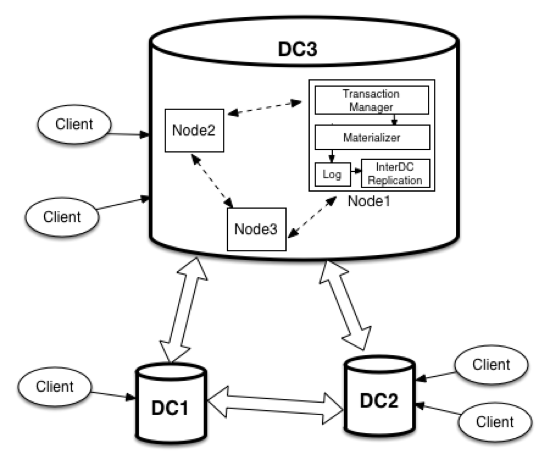
\includegraphics[width=0.9\textwidth]{figures/antidote_architecture}
	\label{antidote}
\end{figure}

In the current state of the system, an application backed up by Antidote can
communicate with a DC thanks to an API available in Java and Erlang, based on
protocol buffers, a language-neutral, platform-neutral mechanism for
serializing structured data. The API connects to a DC with a socket and sends
serialized operation to the server.


\subsection{EdgeAnt}

A user can communicate with Antidote through an API that provides a simple way
to develop applications based on Antidote, but is very basic, providing a way
to connect to a DC and send transactions. A developer who desires to write an
application based on Antidote will have to build important functionalities of
such system, like a cache, handler of network failure, etc...

EdgeAnt is a module, that simplifies the creation of application using
Antidote. It implements the SwiftCloud approach \cite{Zawirski2015} to extend
geo-replication to the client machine, pushing consistency, convergence and
availability guarantees to the client cache.

First it provides a causally consistent subscription service: applications can
subscribe to a set of keys, its interest set, and every time an update occurs
on one of the keys, the data centre notifies the client with the new value.
This way, causal consistency between client cache and updates from other
clients is maintained by the data centre, that we can trust to send only
causally consistent updates.

EdgeAnt can also dynamically switch from a crashed DC to an available one.
Finally, it has the capability to use the data present in the cache to repair
a failed DC. Applications interact exclusively with EdgeAnt in a very
transparent way, because it exposes the same protocol buffer interface as
Antidote. EdgeAnt forward requests to the Antidote server, after passing them
through two components: its state cache and log cache.

\paragraph{State cache:}
The state cache stores the state of the objects from the user's interest set
and every read is performed through this cache. At initialisation, the cache
is filled with the state of all the keys in the interest set. This projection
of the data centre's state into the interest set is necessarily causally
consistent. Afterwards, the state of the client can change because of internal
updates or external updates received from a DC. Internal updates made on a
causally consistent state maintains causal consistency. External updates
coming from other users are pushed by the DC when it makes them visible. We
can trust the DC to send causally consistent updates, so the consistency is
maintained system-wide.

If a read is made on a key not present in the interest set, this key is added
in the set. If there is a cache miss, all the interest set is synced with the
Antidote node. The reason to sync all the interest set and not just read the
missing object is that we want to guarantee causal consistency at every
instant in the cache. If we only read one object, we could miss some causal
dependency.

\paragraph{Log cache:}
The log cache stores every local update. Its goal is to permit the user to
make fast writes by avoiding round-trip with the Antidote node every time. The
principle is that write operations update the state cache, and then are
buffered in the log cache. Later, a background thread sends asynchronously
those updates to the node. Once an operation has been successfully sent to the
DC, it is evicted from the cache. This mechanism makes writes faster, but also
permits offline updates as it is not necessary to be connected to a node to
update the cache. The application can therefore work even in case of network
partition or failed node. The process of an update is as follows: first there
is a check to see if the object is present in the state cache. If it is the
case, the cache is updated, otherwise the state cache is synced with the DC,
like for a read, and then the cache is updated.

Those two caches are implemented with a classical LRU algorithm. If the state
cache is full, then the least recently used object is evicted from the cache,
at the condition that every update on this object on the log cache is sent to
the DC. If the log cache is full, either because the pace of the writes is way
superior than the propagation's speed of the updates to the DC or because the
user is making a lot of write while offline, then the user can not submit any
write until the cache flushes its updates.


\paragraph{Metadata:}\mbox{}
EdgeAnt uses a lightweight metadata design to ensure causal consistency and
at-most-once delivery. Each update is initially associated with a
client-assigned timestamp and a version vector. The client-assigned timestamp
is a pair (clientID, sequence number). ClientID is a unique identifier
provided by the DC when the client starts a session and the sequence number is
used as a timestamp to order updates locally. The version vector encodes the
causal dependencies of an update. It is a snapshot that identify the object
versions present in the state cache. This version vector is in fact the last
Global Stable Snapshot (section \ref{sec:cure}) EdgeAnt saw. EdgeAnt receives
a new GSS in the following cases: when it syncs with the DC following a cache
miss; after an update has been successfully propagated to a DC, the DC sends
an acknowledgment to the client that contains the GSS assigned to this update;
when a DC notifies the client of an external update. 

The log cache sends these two elements with the update during the propagation
to a DC. When a DC receives an update, it checks first if it did not already
apply the update thanks to the client-assigned timestamp, preserving
at-most-once delivery. Then, it checks that it has all the update's internal
and external dependencies. Finally, it assigns the GSS to the update and
stores it locally. The update will later be propagated to the other DC thanks
to Cure replication protocol. As said earlier, the DC terminate the process by
sending an acknowledgment to EdgeAnt with the assigned snapshot.


\paragraph{K-stability:}
A client can switch to a new DC at any time, in particular in response to a
network failure or a crash. Since Antidote provides eventual consistency,
there is no guarantee that an update delivered to the failed DC has been
delivered to the other DCs. To maintain causal consistency, the client must
observe a monotonically increasing progression of replica states. A client
state can not "return in the past" if the new DC missed some updates.
Therefore, availability will be reduced until the failed DC recover and
propagate its updates. SwiftCloud's gives two answers to this problem. First,
it makes the client cache co-responsible for the recovery of missing causal
dependencies at the new DC. This solution is not sufficient, as the cache does
not always contain all the missing dependencies needed to make the DC
available for itself. The other solution brings by Swiftcloud is that the
clients observe only its own updates and the K-stable updates from the other
clients. An update is K-stable if it has been applied in at least K DCs, where
K is configurable. The higher K is, the more we decrease the chance that the
system be unavailable, however the more stale the data will be.


%There will be time where EdgeAnt will be in the future or in the past compare
%to the DC. In the case where the DC is in advance while notifying EdgeAnt with
%new updates, those updates are buffered in EdgeAnt until it receives the
%missing update. In the case where EdgeAnt is beyond the DC while propagating
%updates, the write on the DC is pending until the DC catch up. 

%\subsubsection{Metadata}
%\begin{itemize}
%        \bulletitem Client Local Clock to order the operation within the cache
%        \bulletitem Last known GSS
%        \bulletitem Cache (LRU)
%        \bulletitem interest Set
%\end{itemize}

\section{Contribution}

We presented the current state of the system as studied during this
internship. On the DC-side we have Antidote, a geo-replicated database that
provides strong consistency and convergence guarantees with a high throughput.
On the client side we have EdgeAnt, an extension of Antidote to the Edge that
provides consistent partial replication on a client device, with built-in
failure recovery. Clients can execute fast transactions locally and even
offline. But client side execution is not always beneficial. For instance,
computation that access a lot of data, such as search or recommendations is
better done in the DC.

We had two main objectives during this internship. First, we had to implement
a component placed between EdgeAnt and an Antidote data centre, that would
allow an EdgeAnt client to offload a piece of code to be executed on the
DC-side. The challenge of this first step is to ensure that the result of this
remote execution is the same as that of a local execution. The value returned
by the remote call and the state of the EdgeAnt cache must be the same that if
the code had been executed on the client device. The second step was to choose
and implement a scheduling strategy, that could dynamically decide where to
execute a piece of code.

We failed to reach the second step and did not finish the implementation of
the first step. What will be presented in the following subsection is the
specification of the first step. We present what needs to be added to both
Antidote and EdgeAnt interface, and the design of our solution.

%\subsection{State of the art}
%\begin{itemize}
%	\item Toward a smart job and data placement in grid computing
%	\item CloneCloud: Dinamically send heavy code on the server
%\end{itemize}

\subsection{Code offloading}

This section described the specification of the code offloading module. We
will refer to this module as CO for simplicity. The module can only upload
Erlang code. This code can contain any Erlang built-in method and library. It
can also call method from external libraries, if library has been uploaded
too. The obvious security problems are not addressed in this internship. CO
provides an interface to execute read-only transactions as well. This
interface is duplicated on the client device and on the server. If this
interface is used from the client device, it just executes EdgeAnt read
transactions. If this interface is used from an offloaded code on a server, it
will execute the transaction protocol that we will know describe.

\paragraph{Transaction protocol:}

CO offers the following methods to start a job and build read-only
transactions: $start\_job$, $start\_transaction$, $read\_objects$ and
$commit\_transaction$.

When a client device starts a job remotely, it gives the snapshot on which the
job executes. This snapshot is the last GSS seen by EdgeAnt. The GSS will
permit CO to read data consistent with the cache of EdgeAnt. EdgeAnt also
provides its local clock, so CO can check if it misses updates from this
client. Finally, it gives its current interest set. This is necessary if the
job read an object that is not in this set. In this case, CO will have to
update the interest set on the DC and on the client at the end of the job. 

When $read\_objects$ is called, CO will just ask the objects to Antidote as a
regular client. If there is internal dependencies missing, CO makes a remote
call to fetch them from the client's log cache. It then applies those updates
on the read objects. CO do not transfer these updates to the DC, since it only
provides read-only transactions, it lets EdgeAnt propagate those updates
itself later.

$commit\_transaction$ closes the transaction but does nothing
special since it is a read-only transaction.

\paragraph{Modification of EdgeAnt:}

EdgeAnt can invoke CO while some of its local updates have not been propagated
to the DC. The state of EdgeAnt is therefore in advance compare to the DC. The
reads made on the DC-side must see those updates, otherwise we would violate
the invariant that clients must observe a monotonically increasing progression
of replicas state. A simple solution is to have EdgeAnt synced with the DC
before launching a job execution. This solution could increase the latency
more than necessary by sending updates not necessary for the execution. We
decide that CO will have to ask for missing update to EdgeAnt during the
execution. Therefore, we need to add the following function to EdgeAnt
interface: $get\_updates([Keys], Snapshot) : [Operation]$ \\

\paragraph{Modification of Antidote:}\mbox{}

One of the invariants our module needs to conserve is that an EdgeAnt client
only reads its own updates and the K-stable updates from other clients.
K-stability in EdgeAnt is tracked by a daemon in the client side. The tracking
is made on the client side because one of the goal of EdgeAnt in the long term
is to be able to have user-to-user communication. An application on a user
device will look for data at the device of a client near by instead of
contacting the DC. First, we thought that since our module is executed on the
server side, we needed to add the capability in Antidote to read from a
K-stable snapshot. It was a mistake. An EdgeAnt client provides the last GSS
it saw to CO when it launches an execution. The architecture of EdgeAnt
ensures that this snapshot includes only its own updates and K-stable updates
from other clients. I progressed too much in the solution of this problem
before realising it was not one in our case. We present it here as a
contribution, because it presents a way to modify the Cure protocol to provide
support for K-stability in an asynchronous way. This could be useful if we
want to build a client other that EdgeAnt, that did not want to handle
K-stability in the client-side.

To that end, we modify the Cure protocol explained in \ref{sec:cure}. We keep
the mechanism of the Global Stable Snapshot and add a new Global K-stable
Snapshot (GKSS).

We present the modification made to the Cure protocol to track K-stable
updates. In the following pseudocode (Algo \ref{algo:kstability-protocol}), we
have a lighter version of the Cure protocol presented in \cite{Cure2016}. We
trim the code to the part necessary for replication between DC on the one hand
and the computation of a Global Stable Snapshot by a partition on the other
hand.

First, we explain the part of this pseudocode that is in Cure. The third row
of Table \ref{table:notation_protocol} is added for our contribution and is
not considered for the moment. We recall that in Cure, the database is
partitioned and geo-replicated, we note $p_d^m$ the partition $m$ in DC $d$.
The propagation of updates between replicas is made at the partition level.

In the function \textbf{propagate\_transaction}, we can see how sibling
partitions periodically communicate to send their local progress, i.e. local
updates associated with a commit timestamp $ct_T$ or just a heartbeat if there
have been no updates. We note $pvc_d^m$ the version vector maintains by the
partition $m$ at DC $d$. The entry of index $i$ reflects the progress made by
the partition $p_i^m$ received by $p_d^m$, except for the entry $m$ which
represents the progression of $p_d^m$. This version vector is updated when a
partition receives a heartbeat or a remote update. The entry $m$ is
incremented by the partition when it propagates update, but it is not shown
here to simplify. When a partition sends a heartbeat, it just sends this
vector as seen in line 11. In the functions \textbf{heartbeat} and
\textbf{replicate\_transaction}, we can see how $pvc_d^m$ is updated, line 19
and 23. Now, the Cure protocol needs to decide which remote updates can be
made visible. To that end, partitions within a DC periodically send their
$pvc$. A partition $m$ maintained the matrix $PMC_d^m$ of all the received
$pvc$ and compute the $GSS_d^m$ as the aggregate minimum of all $pvc$. we can
see the periodic propagation of $pvc$ in \textbf{bcast\_pvc} and the
computation of $GSS_d^m$ in \textbf{update\_GSS} line 41-42.

Now, we explain the pseudocode of our contribution to add K-stability in the
protocol. We keep the GSS as it is because, we let the possibility to a user
of Antidote that is not EdgeAnt to read no K-stable version. We recall that an
update is K-stable if $K$ DCs received it, K being a configurable number.
Since in Cure the propagation of updates is made at the partition level, this
is the role of the partitions to detect when an update is K-stable. Then,
partitions compute a GSS of K-stable updates, called $GKSS$, in the same way
we saw earlier. Intuitively, $GKSS$ is equal to $GSS$ if $K$ = 1. First, we
explain the algorithm made by a partition to compute a local K-stable
snapshot, implemented by the function \textbf{compute\_pkvc}. When a partition
$p_d^m$ received a snapshot (a version vector) from a sibling partition, it
saved it in a matrix $PMRemote_d^m$. This matrix has $M$ rows and $D$ columns
and is initialized to zero line 3. To simplify the code, we define a function
$kmax$ that takes a vector and returns the $k^{th}$ biggest element, $k$ being
the configuration chosen for the K-stability. For example, for $K$ = 2 and a
vector [11, 7, 5], $kmax$ return 7, the $2^{th}$ biggest element.

Here an example of computation of K-stability to clarify: We have a system of
3 interconnected data centres, each having M partitions (not important here)
and $K$ is fixed at 2. We place ourselves in the DC $1$ on the partition $2$
noted $p_1^2$.
\setcounter{equation}{0}
\begin{gather}
	p_1^2 \ has\ a\ pvc = [11, 4, 2]; \\
	p_1^2\ received\ [7, 7, 3]\ and\ [4, 5, 3]\ from\ siblings\ p_2^2\ and\ p_3^2\\
	PMRemote_1^2\ =
	\begin{bmatrix} 
	11 & 4 & 2\\
	7 & 7 & 3\\
	4 & 5 & 3 
	\end{bmatrix} \\
	kmax\ with\ K = 2\ applied\ to\ each\ columns\ returns\ [7, 5, 3] \\
	pkvc_1^2 = min([11, 4, 2], [7, 5, 3]) = [7, 4, 2]
\end{gather}\\

\begin{itemize}
	\bulletitem (1): [11, 4, 2] is the consistent view available at $p_1^2$,
	it means that it receives updates until snapshot 4 for $p_2^2$ and until
	2 for $p_3^2$ and its current advancement is 11.
	\bulletitem (2): $p_1^2$ received heartbeats from siblings partitions.
	\bulletitem (3): $p_1^2$ updates $PMRemote_1^2$ accordingly. The first
	column is the progress of $DC_1$ available in the 3 DCs, the second column
	the progress of $DC_2$, etc...
	\bulletitem (4): $kmax$ is applied on each column of the matrix and
	returns [7, 5, 3], this vector is a snapshot containing updates which are
	2-stable between partition $p^2$ replicas.
	\bulletitem (5): The previous vector is not sufficient, we can see that
	the second entry 5 is not available at $p_1^2$ which is still at 4. So we
	compute the minimum between $pvc_1^2$ and the k-stable vector. The vector
	$pkvc_1^2$ obtained reflects the k-stable updates available at $p_1^2$.
\end{itemize}

This is how partitions compute k-stable vectors. We can see that there is a
gap between $pvc_1^2$ ([11, 4, 2]) and $pkvc_1^2$ ([7, 4, 2]). Reading from
K-stable updates increases staleness as said earlier. Afterwards, partitions
can compute the GKSS the same way they do the GSS, as seen in line 40 and 43.

\newcommand*{\myalign}[2]{\multicolumn{1}{#1}{#2}}

\begin{table}[H]
	\begin{tabular}{ c|c }
		\hline
		\myalign{r}{M} & \myalign{l}{Number of partitions at a data centre}\\
		\myalign{r}{D} & \myalign{l}{Number of data centres in the system}\\
		\hline
		\myalign{r}{$p_d^m$} & \myalign{l}{Partition $m$ at DC $d$}\\
		\myalign{r}{$pvc_d^m$} & \myalign{l}{Version vector at partition $p_d^m$ -> updates received from siblings }\\
		\myalign{r}{$PMC_d^m$} & \myalign{l}{Matrix of received $pvc_d^i$ to compute GSS at $p_d^m$}\\
		\myalign{r}{$GSS_d^m$} & \myalign{l}{Global Stable Snapshot of $p_d^m$, a version vector}\\
		\hline
		\myalign{r}{$PMRemote_d^m$} & \myalign{l}{Matrix of remote $pvc_d^i$ received to compute $pkvc_d^m$}\\
		\myalign{r}{$pkvc_d^m$} & \myalign{l}{Version vector at partition $p_d^m$ -> k-stable updates received from siblings}\\
		\myalign{r}{$PMKC_d^m$} & \myalign{l}{Matrix of received $pkvc_d^i$ from partitions of the DC to compute GKSS at $p_d^m$}\\
		\myalign{r}{$GKSS_d^m$} & \myalign{l}{Global K-Stable Snapshot of $p_d^m$}\\
		\hline
		\myalign{r}{$T$} & \myalign{l}{Transaction}\\
		\myalign{r}{$ct_T$} & \myalign{l}{Version vector assigned as $T$'s commit snapshot}\\
		\myalign{r}{$committedTx_d^m$} & \myalign{l}{Set of committed transactions at $p^m_d$}\\
		\myalign{r}{$ws_T[m]$} & \myalign{l}{Set of updates made in transaction T by partition m}\\
		\hline
	\end{tabular}
	\caption{Notation used in the protocol description}
	\label{table:notation_protocol}
\end{table}

\newpage
\thispagestyle{empty}


\def\myspace#1{%
  \foreach \index in {1, ..., #1} {%
	$\ $
}}
\algtext*{EndFor}% Remove "end for" text
\algtext*{EndFunction}% Remove "end function" text
%\algtext*{EndIf}% Remove "end if" text

\algnewcommand{\Initialize}[1]{%
  \State \textbf{Init:}
  \Statex \hspace*{\algorithmicindent}\parbox[t]{.8\linewidth}{\raggedright #1}
}

\begin{algorithm}[H]
	\begin{algorithmic}[1]
		\caption{Cure protocol with K-stability executed at partition $p_d^m$}
		\label{algo:kstability-protocol}
		\State \textbf{Init:}\\
		$pkvc^m_d[i] \gets 0, i = 1...D$\\
		$PMRemote_d^m[i] \gets pkvc^m_d, i = 1...D$\\
		$PMKC_d^m[i] \gets pkvc^m_d, i = 1...M$\\
		$GKSS^m_d[i] \gets 0, i = 1...D$\\
					
		\Function{$\textbf{PROPAGATE\_TRANSACTION}$}{\mbox{}}\myspace{4} $\triangleright$ Run periodically
			\If{$committedTx_d^m = \emptyset$}
				\For{$k = 1...D, k \neq d$}
					\State send HEARTBEAT($pvc_d^m, d$) to $p_k^m$ \label{algo:send_heartbeat}
				\EndFor
				\Return
			\EndIf
			\ForAll{$\langle T, ws_T[m], ct_T \rangle \in committedTx_d^m$}
				\For{$k = 1...D, k \neq d$}
					\State send REPLICATE\_TRANSACTION($ws_T[m],ct_T,d$) to $p_k^m$ 
					\State $committedTx_d^m\ \gets committedTx_d^m\setminus\{T\}$
				\EndFor
			\EndFor
		\EndFunction\\

		\Function{$\textbf{HEARTBEAT}$}{$pvc, k$}
			\State $pvc_d^m[k] \gets pvc[k]$ \label{algo:heartbeat_update}
			\State COMPUTE\_PKVC($pvc, k$)
		\EndFunction\\

		\Function{$\textbf{REPLICATE\_TRANSACTION}$}{$ws_T[m],ct_T,k$}
			\State $pvc_d^m[k] \gets ct_T[k]$ \label{algo:remote_tx_update}
			\State COMPUTE\_PKVC($ct_T, k$)
		\EndFunction\\

		\Function{$\textbf{COMPUTE\_PKVC}$}{$snapshot, k$}
			\State $Temp[i] \gets 0, i = 1...D$ // Temporary vector
			\State $PMRemote_d^m[d] \gets pvc_d^m$
			\State $PMRemote_d^m[k] \gets snapshot$
			\For{$k = 1...D, k \neq d$}
				\State $Temp_d^m[k] \gets \kmax\ applied\ to\ column\ k\ of\ PMRemote_d^m$
			\EndFor
			\State $pkvc_d^m \gets \min\limits_{i = 1..D}(pvc_d^m[i], Temp[i])$
		\EndFunction\\

		\Function{$\textbf{BROADCAST\_PVC}$}{\mbox{}}\myspace{14} $\triangleright$ Run periodically
			\ForAll{$i = 1...M$}
				\State send UPDATE\_GSS($m, pvc_d^m, pkvc_d^m$) to $p_d^i$
			\EndFor
		\EndFunction\\

		\Function{$\textbf{UPDATE\_GSS}$}{$i, pvc, pkvc$}
			\State $PMC_d^m[i] \gets pvc$
			\State $PMKC_d^m[i] \gets pkvc$
			\For{$k = 1...D, k \neq d$}
				\State $GSS_d^m[k] \gets \min\limits_{i = 1..M} PMC_d^m[i][k]$
				\State $GKSS_d^m[k] \gets \min\limits_{i = 1..M} PMKC_d^m[i][k]$
			\EndFor
		\EndFunction

	\end{algorithmic}
\end{algorithm}


%\subsection{API provided by the contribution}
%
%Placed on the device hosting EdgeAnt. This API provides the capability to send
%requests to the CodeMoving module located on the Antidote node, hiding the
%boilerplate of serializing objects and sending in the network. All those
%requests are synchronous, so the caller wait until it receives a response. To
%avoid waiting indefinitely a thread will check the liveness of a DC with a
%heartbeat.
%
%%It will also maintain for each connection the following data:
%%\begin{itemize}
%%    \bulletitem Obviously, the socket for the connection
%%	\bulletitem The last GSS seen by the client
%%\end{itemize}
%
%Here is the interface offered to EdgeAnt:
%\begin{itemize}
%        \bulletitem $connect(ip\_addr, port, ClientID) : ConnectionID$
%		\\Create a connection with an Antidote node and return the tuple
%		\{Socket, ClientID\}, ClientID is the unique identifier of the client
%		provided to EdgeAnt by the DC at first connection.
%		\bulletitem $start\_transaction(ClientID, Snapshot, InterestSet) : TransactionID | error$
%		\\Start a transaction with the given Snapshot. Create an instance of a
%		transaction manager and a cache for the client. It syncs with the DC
%		to be sure that it has received every local update up to Timestamp.
%		It returns the id of the transaction that should be used in following
%		called of $read\_objects$ and $commit\_transaction$.
%		It is a pair (ClientID, TxID), with TxID a structure provided by the
%		DC.
%        \bulletitem $read\_objects(ClientID, TransactionID, [Keys]) : Value \parallel ok$
%        \\Read the list of objects associated with the keys $Keys$, one element of
%        Keys is a tuple in the form $\{key, crdt\_type, bucket\}$
%        \bulletitem $commit\_transaction(ClientID, TransactionID) : CommitSnapshot$
%        \\Commit the transaction and return the Snapshot of the commit, which
%        became the new GSS of the client.
%        \bulletitem $store\_module(ClientID, Module): ok \parallel error$
%        \bulletitem $start\_job(ClientID, Module, Function, Args) : ok \parallel error$
%        \\Execute a remote procedure call, with a module that has been previously
%		charged with $store\_procedure$. The function must take only one list
%		as argument.
%        \bulletitem $disconnect(ClientID)$
%        \\Close the communication with the DC.
%\end{itemize}

%\subsubsection{Interface needed by the contribution}
%
%$update\_interest\_set((Scalar, DCID), InterestSet) : ok \parallel error$ \\
%Both EdgeAnt and the Antidote node must provide this method. Every time
%EdgeAnt executes a read on a key not present in its interest set, EdgeAnt
%updates it with this new key. If the read is executed on the DC-side, then it
%can not perform those changes. So EdgeAnt needs to provide this function
%allowing the CodeMoving module to let it know that it has to update its
%interest set. The Antidote node must provide this function as well, since it
%has a copy of the interest set, used to notify EdgeAnt every time an update on
%one of those keys is committed.
%
%\subsubsection{Pseudocode}
%
%\begin{algorithm}
%	\caption{Protocol executed at client side}\label{client side-code}
%	\begin{algorithmic}[1]
%		\Function{$\textbf{CONNECT(ip\_addr, port)}$}{}
%			\State $Socket \gets connect(addr, port)$
%			\If{$Socket = error$}
%				\State \Return error
%			\EndIf
%			\State generate SocketID and store the association SocketID => Socket
%			in connection pool
%			\State send $connect()$ to Socket
%			\State (Scalar, DCID) $\gets $ wait ClientID from Socket
%			\State \Return (Scalar, DCID)
%		\EndFunction.
%
%
%		\Function{$\textbf{START\_TRANSACTION(ClientID, Snapshot, InterestSet)}$}{}
%			\State call \textbf{edgeant\string:sync()}
%			\State $Socket \gets$ retrieve socket matching SocketId
%			\State $(Scalar, DCID) \gets$ extract from ClientID
%			\State Send $start\_transaction((Scalar, DCID), Snapshot, InterestSet)$ to Socket
%			\State TransactionID $\gets$ wait response from $Socket$
%			\State \Return TransactionID
%		\EndFunction.
%	\end{algorithmic}
%\end{algorithm}
%	
%
%\begin{algorithm}
%\caption{Protocol executed at server side}\label{server side code}
%	\begin{algorithmic}[1]
%		\Function{$\textbf{START\_TRANSACTION((Scalar, DCID), Snapshot, InterestSet)}$}{}
%			\State send $start\_transaction(Snapshot, [Properties])$ to the DC
%			\State $TxID$ $\gets$ wait for response from DC
%			\State initiate the transaction manager process
%			\State initiate the cache process
%			\State $state.interest\_set \gets InterestSet$
%			\State $state.ops\_buffer \gets \emptyset$
%			\State \Return TxID
%		\EndFunction
%
%		\Function{$\textbf{read\_objects(ClientID, TransactionID, [Keys])}$}{}
%			\State $Snapshot$ $\gets$ extract Snapshot from TransactionID
%			\State $Values$ $\gets \emptyset$ 
%			\ForAll{$Key \in Keys$}
%				\If{$Key \in$ cache with version $Snapshot$}
%					\State $Val \gets $ cache[$Key$]
%				\Else
%					\State $Val \gets $ send $read\_key(Snapshot, Key)$ to DC
%					\State cache $\gets$ cache $\cup\ [Key \mapsto Val]$
%				\EndIf
%				\If{$Key \notin state.interest\_set$}
%					\State $state.interest\_set \gets state.interest\_set \cup \{Key\}$
%				\EndIf
%				\State $Values \gets Values \cup \{Val\}$
%			\EndFor
%			\State \Return $Values$
%		\EndFunction.
%
%		\Function{$\textbf{commit\_transaction(ClientID, TransactionID)}$}{}
%		\EndFunction.
%	\end{algorithmic}
%\end{algorithm}
%
%The figure \ref{contribution} presents the architecture of the system once our
%contribution is integrated.
%
%\begin{figure}[ht]
%	\caption{Architecture of an Antidote system which include my contribution.}
%	\centering
%	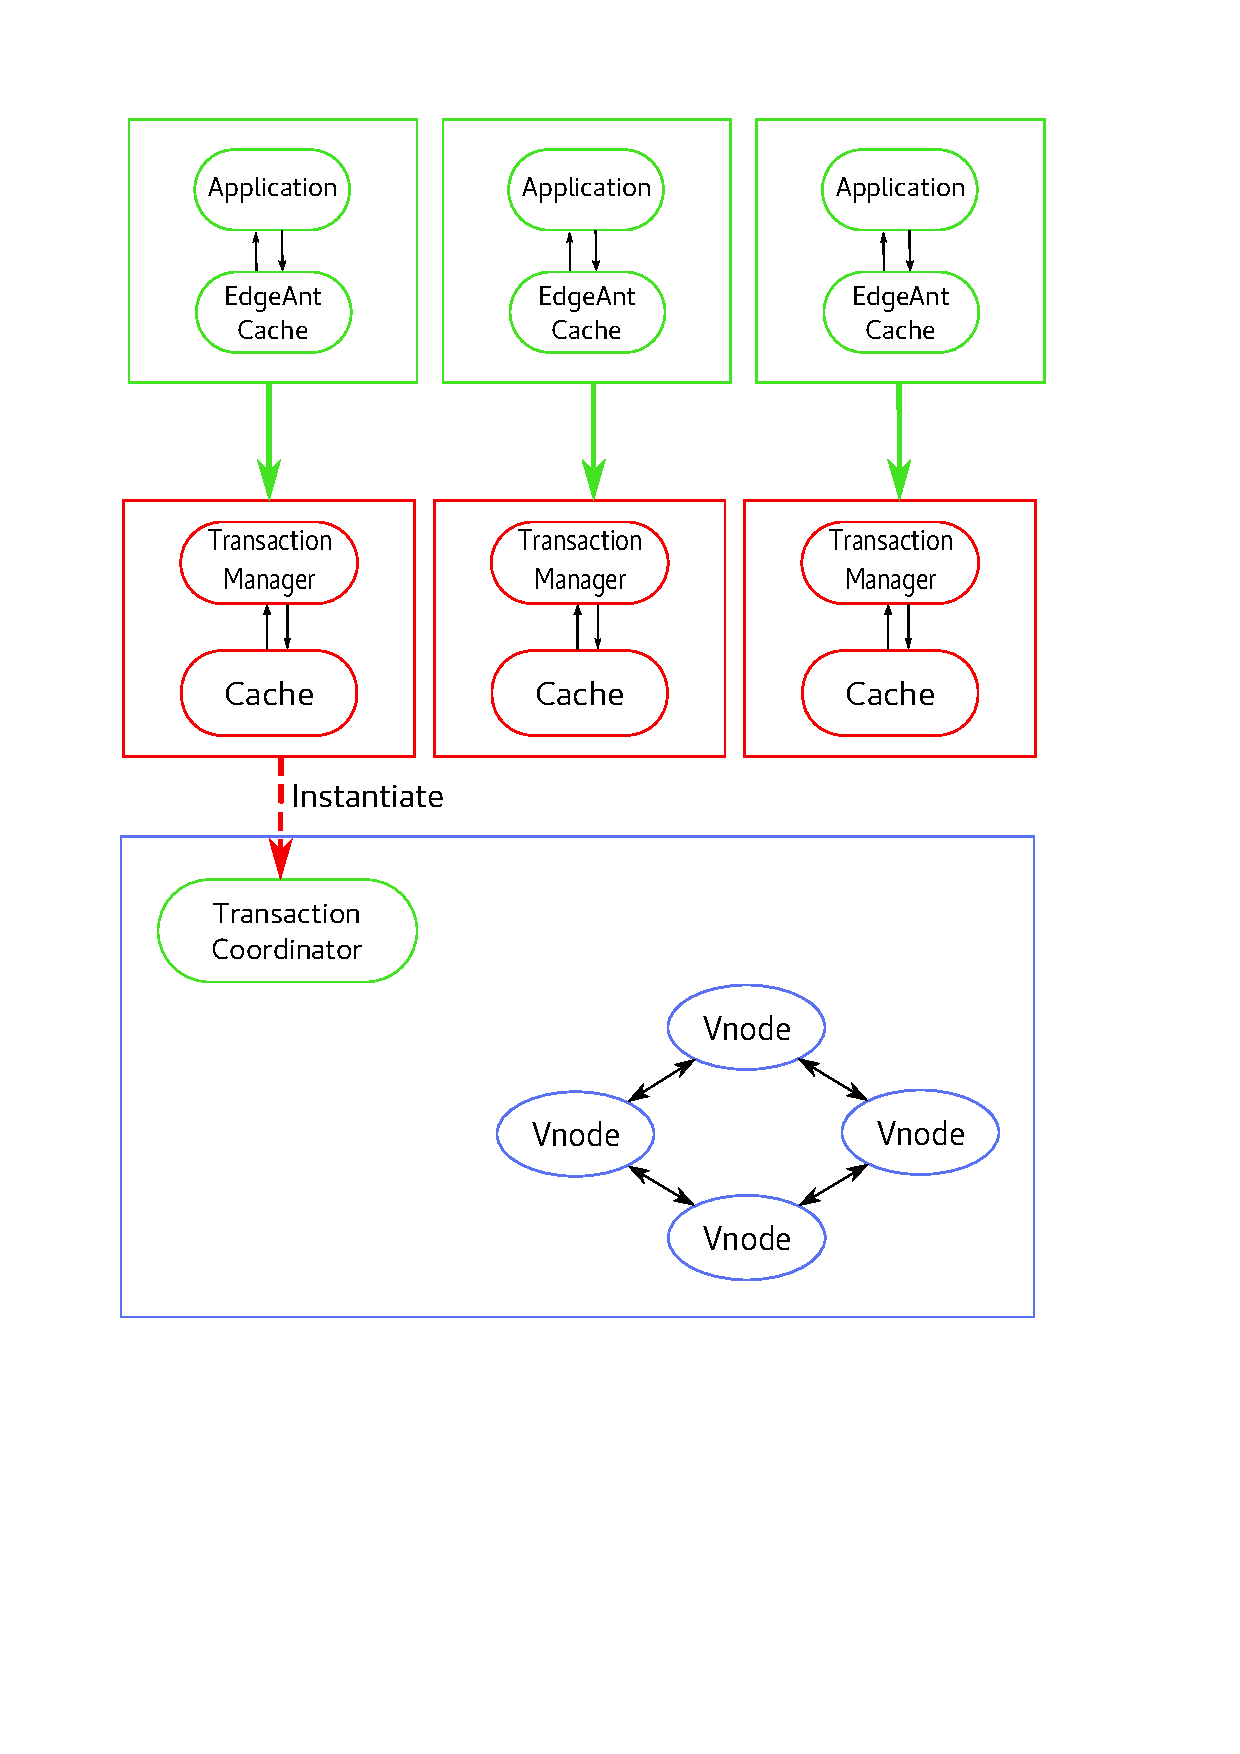
\includegraphics[width=0.9\textwidth]{internship_architecture}
%	\label{contribution}
%\end{figure}

%\section{Limitations}
%\textbf{Trade Off:} Instantiate module for each transaction, or maintain a
%cache as long as the client did not close the connection.
%=> Easier but more round-trip with the dc/more sync to maintain consistency.
%
%\begin{itemize}
%        \bulletitem Can not prevent recursion
%        \bulletitem Security problem: access to filesystem/memory (use docker ?)
%\end{itemize}
%

%\section{Evaluation}
%
%In this section we describe the test needed to evaluate our contribution.
%Those tests are based on FMKe, an application benchmark created to evaluate
%geo-replicated key-value stores providing weak consistency \cite{FMKE2017}. It
%is based on a real system: the Danish National Joint Medicine Card (FMK for
%Faelles Medicinkort). Implementation of the benchmark exists for Antidote, so
%this is the one we chose to evaluate our contribution.
%
%\subsection{Correctness test}
%
%Ensure to have the same log with or without the contribution at the end of
%the benchmark.
%
%\subsection{Performance test}
%
%Test the performance of the contribution with different workload and
%configuration (1 client/1 DC, N clients/N DCs, N clients/N Dcs). Obtain few
%scenarios where the performance with CodeMoving or superior that the one
%without. Have a scenario where the performance with CodeMoving are inferior,
%hopefully not too much.
%
%\subsection{Causality Test}

\section{Future Work}
As said in the previous section, we only started to think about the solution
and its specification, when we reached the end of this internship. There is a
lot of refining to do in the transaction protocol and off course it needs to
be implemented and tested.

For the evaluation, we wanted to use FMKe, an application benchmark created to
evaluate geo-replicated key-value stores providing weak consistency
\cite{FMKE2017}. It is based on a real system: the Danish National Joint
Medicine Card (FMK for Faelles Medicinkort). Using the data and access pattern
of a realistic application provides relevant performance evaluation.
Implementation of the benchmark exists for Antidote, so it seems like a good
choice to evaluate the performance of our contribution and compared it to the
current system. FMKe can be used to test a database in term of throughput or
latency. To evaluate our work properly we also need to define consistency
tests, especially in the presence of network partitions, but we haven't
thought about how to create those tests.

The second step, after developing a fully functional code offloading module,
is to integrate a scheduler in EdgeAnt. The goal is to dynamically determine
if a piece of code should execute on the client device or on a data centre. We
start looking in the domain of cyber foraging (\cite{Cyberforaging2017}).
Searchers in this field try to find efficient solution to offload code from a
mobile device to nearby servers. The main challenge is to properly partition
the application into pieces that can seamlessly be offloaded to a remote
server. Pieces of an application well-suited for remote execution are parts
that do not depend on external input, like input from an user or information
from the material. Secondly, some side-effect must be avoided like writing on
disk or modify the user interface. Finally, sending the request and its
arguments and receiving its result should have a significantly lower cost than
the perceived latency if the request had been executed on the client device.
MAUI \cite{MAUI:2010} for example, lets the developer decides which methods of
an application are safe for remote execution with a special annotation. It
handles the problem of executing the code on different type of architecture by
using the Microsoft .NET Common Language Runtime, which means it only support
applications coded in language support by this runtime like C\#. Similarly,
CloneCloud\cite{CloneCloud:2011} runs on a modify JVM, and can support
application coded in Java. In CloneCloud a static analysis of the application
determines which method can be offloaded. Finally, our code offloading module
runs on the Erlang virtual marchine and takes advantage of a language
capability to unload binary code to a remote Erlang VM. We would probably
choose the same solution of MAUI and let the developer defines which method
can be offloaded.

Once the partitioning is done, the second challenge is to determine
dynamically when an update must be executed on the client device or on a
remote server. MAUI and CloneCloud dynamically takes this decision by
profiling the application during the execution. They evaluate the "hot part"
in terms of energy consumption or latency and check the current state of the
device such as the battery level or the quality of the network connection
among other things. We have not given much thought to this part of the problem
extensively and it would be interesting to work on a solution for our use
case.




\section{Conclusion}

At the beginning of our internship, we were assigned a different subject. Our
first subject was to create a novel JSON op-based CRDT. Adding the capability
to store JSON documents in the form of a CRDT would make of Antidote a
powerful document store. The second part of this subject was to create a query
language to manipulate those documents in an expressive way. We can think of
point queries on text attribute or interval queries on numerical attribute for
example. To make those queries efficient, support for secondary indexes must
be added in Antidote. Working on this subject for two months, we studied the
theory behind Antidote: The trade-off between consistency and availability
explain in the CAP theorem \cite{CAP:1}, and the related work on consistency
model, placing at different level of this trade-off. Off course, we studied
CRDTs and explored ways to represent a document with an op-based CRDT
(\cite{Martin2012,Kleppmann2016}). And finally, we studied transaction models
to understand the Cure protocol used by Antidote.

This subject has changed for the one we presented in this report. The reason
was that other people had already work on it and it was more a technical
challenge than a research one, so we lost interest for it. In this new
subject, we wanted to add the possibility in Antidote to store code in a data
centre. A developer could use this feature to store parts of an application
that invokes heavy transactions. Those transactions would be executed on the
DC side, which would avoid round-trip with the client and increase performance
as explained in the introduction. Finally, we had the idea to extend this
functionality to enable a client to decide dynamically if a piece of code must
be executed on the client device or on a data centre. We needed to add the
possibility to transfer code between a client device and an Antidote data
centre. We wanted the result of this execution to be the same independently of
where it originated. As said earlier, in our view of the system, a client is a
device hosting EdgeAnt that communicates with one or more Antidote centre. To
understand EdgeAnt, we needed to understand the issue of maintaining
consistency guarantees between a data centre and a partial replica of the
database pushed to the Edge.

In conclusion, during this internship, I study a wide range of academic work
in the field of distributed databases. Consistency model, transaction
protocol, partial replication to the Edge and code offloading to the Cloud; it
was very challenging to place myself in those different research studies. I
most certainly underestimated the difficulty to assimilate all those notions
and did not correctly planned my work. By focusing on smaller objectives and
communicating more with my advisors instead of working in isolation, I would
probably have a better contribution to the Antidote project. It was
nevertheless a pleasant experience in the world of research.

\newpage
\bibliography{bibliography}
\end{document}
